\documentclass[xcolor=dvipsnames]{beamer}

\usepackage[italian]{babel}
\usepackage[utf8]{inputenc}
\usepackage[T1]{fontenc}
\usepackage{color}
\usepackage{hyperref}
\usepackage{graphicx}
\usepackage{floatflt}
\usepackage{float}
\graphicspath{{images/}}
\usepackage{eurosym}
\usepackage{colortbl}
\usepackage{color}
\raggedbottom
\usetheme[currentsubsection]{PaloAlto} 
\usecolortheme{seahorse}
\setbeamertemplate{footline}[frame number]
\setbeamertemplate{items}[ball] 
\setbeamertemplate{blocks}[rounded][shadow=true] 
\title{CPNetSolver}
%\subtitle{}
\author{Francesco Burato, Simone Carriero}
\institute[UNIPD]{
  Dipartimento di Matematica\\
  Università degli Studi di Padova\\[1ex]
  %\texttt{lambdaset@gmail.com}
}
\date{12 Settembre 2013}
\newcommand{\firstFrame}[1]{
\begin{frame}
  \begin{block}{CPNetSolver}
    \begin{center}
    #1
    \end{center}
   \end{block}
\end{frame}
}
\begin{document}

%--- the titlepage frame -------------------------%
\begin{frame}[plain]
  \titlepage
\end{frame}

\section{Introduzione}
\begin{frame}{Introduzione}

Cos'è CPNetSolver
\begin{itemize}
  \item risoluzione di CP-Net
  \item visualizzazione grafo dell'ordine degli assegnamenti
  \item accetta anche CP-Net cicliche
\end{itemize}
\end{frame}

\begin{frame}{Introduzione}

Funzionamento:
\begin{itemize}
  \item accettazione CP-Net in input
        %(DIRE:grammatica pross. slide)
  \item conversione da CP-Net a CSP
  \item calcolo e visualizzazione soluzioni ottime
  \item generazione e visualizzazione grafo dell'ordine degli assegnamenti
\end{itemize}

Idea iniziale:
\begin{itemize}
  \item strumento didattico!
  %(DIRE:in ciascun momento si può cambiare la CP-Net
  %corrente e vedere come cambiano le soluzioni e gli ordinamenti)
  
\end{itemize}
\end{frame}

\begin{frame}[fragile]{Introduzione}

Grammatica
\begin{itemize}
\item
\begin{verbatim}
var X dependsOn={}
dom={x,!x}
:x>!x

var Y dependsOn={}
dom={y,!y}
:y>!y

var Z dependsOn={X,Y}
dom={z,!z}
x,y:z>!z
x,!y:!z>z
!x,y:!z>z
!x,!y:!z>z
\end{verbatim}
\end{itemize}
\end{frame}


\section{Progettazione}
\begin{frame}{Suddivisione architetturale}
\begin{itemize}
  \item package \texttt{constraintobj}
  \item package \texttt{solver}
  \item package \texttt{gui}
\end{itemize}
\end{frame}

\begin{frame}{Rappresentazione dei domini}

\begin{itemize}
  \item class Domain
  \begin{itemize}
    \item[-] accepted: Set[String]
    \item[+] contains(elem: String): Boolean
  \end{itemize}
\end{itemize}
\end{frame}

\begin{frame}{Rappresentazione dei vincoli}
\begin{itemize}
  \item class Constraint
  \begin{itemize}
    \item[-] vars: Array[String]
    \item[-] accepted: List[Array[String]]
    \item[+] projection(variable: String): Set[String]
    \item[+] reduction(variable: String, value: String): Constraint
  \end{itemize}
\end{itemize}
\end{frame}

\begin{frame}[fragile]{Esempio di oggetto constraint}
\begin{verbatim}
c = Constraint(vars     =>  [X, Y, Z]
               accepted => [[0, 0, 1],
                            [0, 1, 1],
                            [0, 1, 0]])
                            
c.projection(X) = [0]
c.projection(Y) = [0, 1]

c.reduction(Y,1) = Constraint(vars     =>  [X, Y, Z]
                              accepted => [[0, 1, 1],
                                           [0, 1, 0]])
\end{verbatim}  
\end{frame}

\begin{frame}{Rappresentazione degli ordini - 1}
\begin{itemize}
  \item class Order
  \item \textbf{Rappresentazione ad albero}: nodi interni per gli assegnamenti, foglie per gli ordini
  \pause
  \item class Comparator per l'accesso
  \item Complessità dipendente dalla \textbf{ricerca nei nodi interni}
  \begin{itemize}
  	\item Ricerca lineare: $O(|dom(V_1)|+\ldots+|dom(V_n)|)$
  	\item Ricerca binaria: $O(log(|dom(V_1)|\cdot \ldots \cdot|dom(V_n)|))$
  	\item Tabella hash:    $O(1)$
  \end{itemize}
\end{itemize}
\end{frame}

\begin{frame}{Rappresentazione degli ordini - 2}
Esempio

\texttt{var A dependsOn=\{B,C,D\}}  \texttt{dom=\{...\}}\\
\texttt{var B dependsOn=\{\}}       \texttt{dom=\{$b$,$\overline{b}$\}}\\
\texttt{var C dependsOn=\{\}}       \texttt{dom=\{$c$,$\overline{c}$\}}\\
\texttt{var D dependsOn=\{\}}       \texttt{dom=\{$d$,$\overline{d}$\}}\\
\begin{center}
  \begin{figure}[ht]
    \centering
    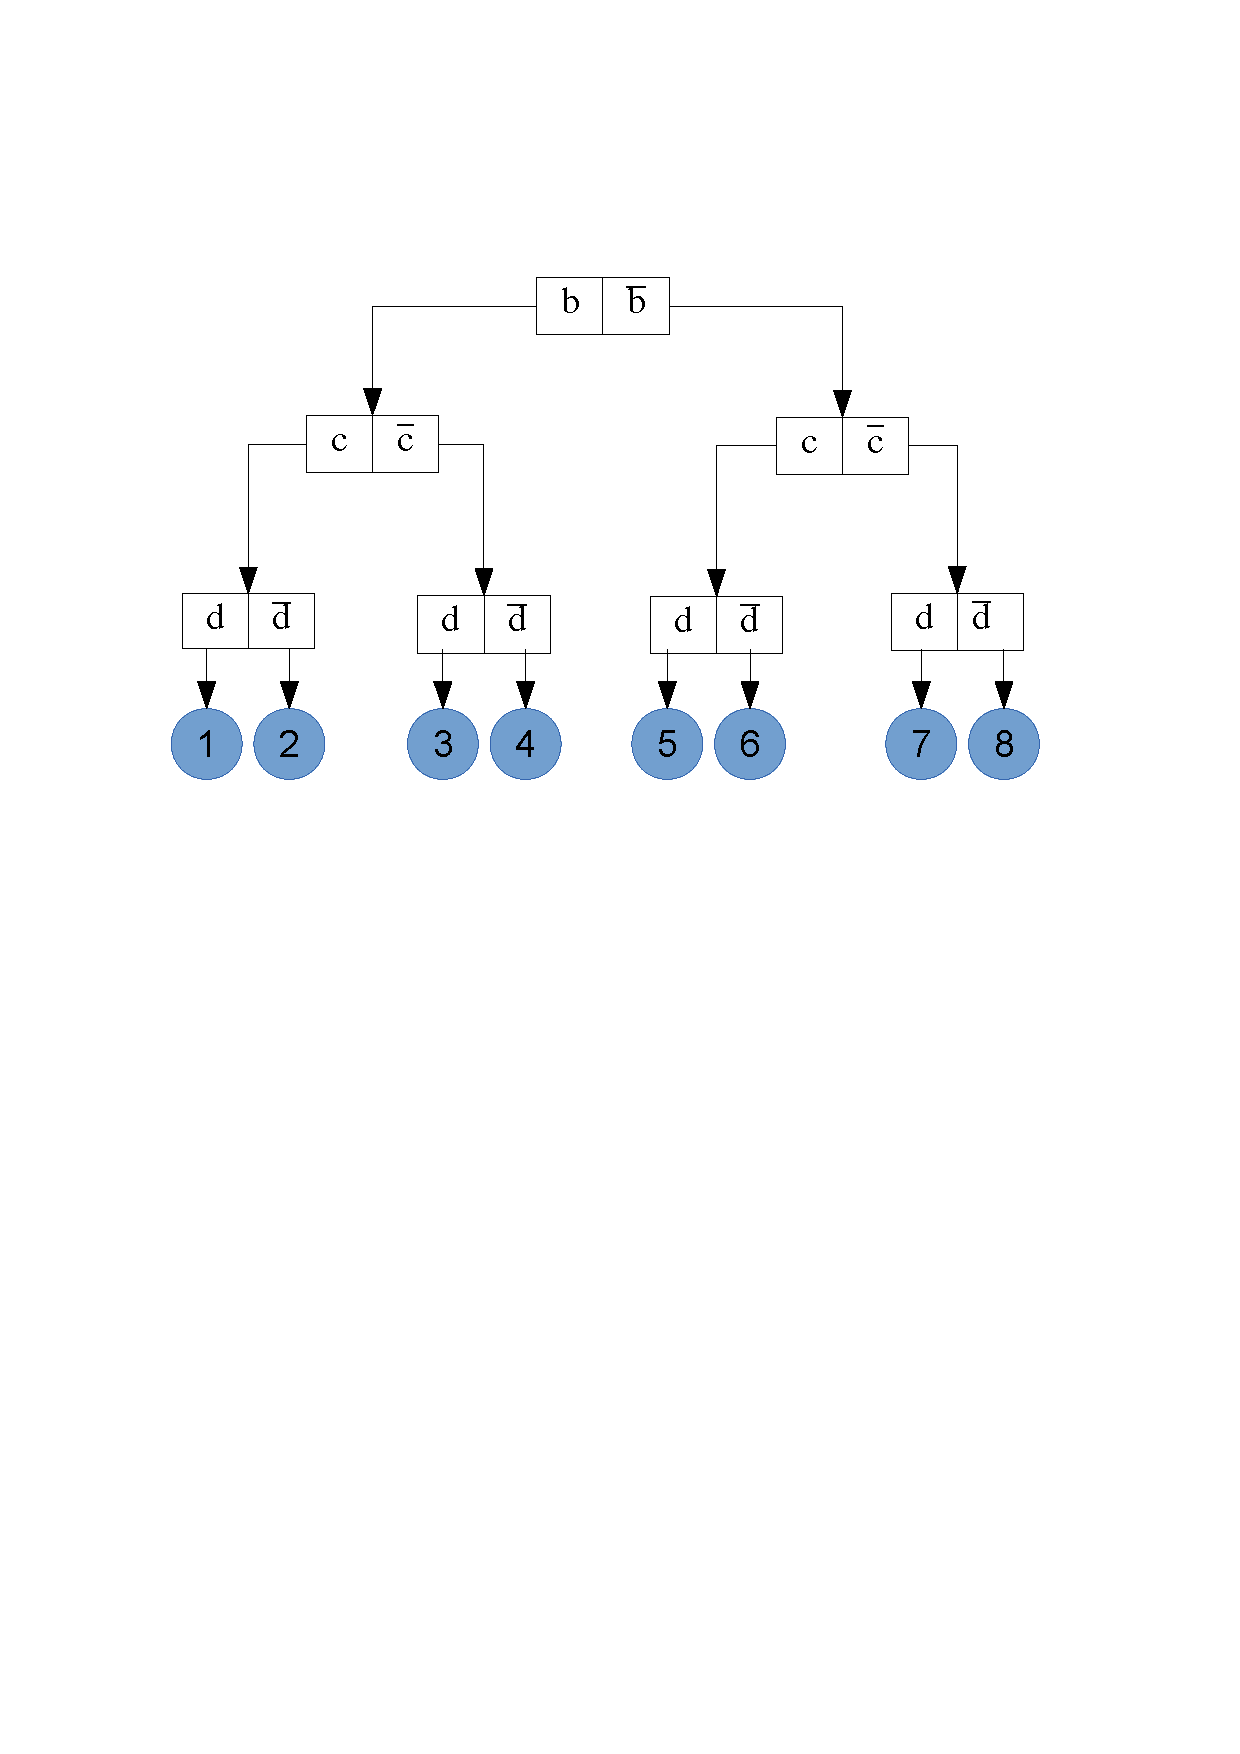
\includegraphics[width=0.5\textwidth]{images/grafo-ordini}
    \caption{\textit{Rappresentazione a grafo di A, B, C, D}}
  \end{figure}
\end{center}
\end{frame}

\section{Algoritmi}

\subsection{Trasformazione da CP-Net a CSP}
Come accennato in precedenza, la ragione per cui si ha la necessità di
trasformare la CP-Net in un CSP è che l'applicazione permette la risoluzione di
CP-Net cicliche, e per la risoluzione di questo tipo di CP-Net è necessario
effettuare tale trasformazione.

Data una CP-Net è sempre possibile costruire un CSP classico con lo stesso
insieme di soluzioni ottime nel seguento modo: per ogni ordine $X_1=x_1, ...,
X_n=x_n: Y=y_1 > Y=y_2 > ... > Y=y_k$ costruiamo il vincolo $X_1=x_1, ..., X_n=x_n
=> Y=y_1$.

Vista la rappresentazione adottata per gli ordini, questo corrisponde a creare, per
ciascuna variabile $v$, un vincolo per ogni foglia dell'albero degli ordini di $v$.
Infatti, considerato che per ogni foglia si conosce l'istanziazione delle variabili
$X_1=x_1, ..., X_n=x_n$ che è rappresentata da tutti i nodi tra la radice e la
foglia, e il relativo ordine $Y=y_1 > Y=y_2 > ... > Y=y_k$
è possibile costruire il vincolo $X_1=x_1, ..., X_n=x_n => Y=y_1$.

\subsection{Ricerca delle soluzioni}
La ricerca delle soluzioni della CP-Net è fatta attraverso un
algoritmo di tipo Backtracking+Forward Checking modificato per trovare
tutte le soluzioni ottime e non solo una soluzione.

L'algoritmo seguito per risolvere un problema a $m$ variabili è quindi
il seguente:
\begin{enumerate}
\item \textbf{Inizializzazione:} Si raccolgano tutti i domini di tutte
  le variabili del problema e tutti i vincoli ottenuti dalla
  conversione della CP-Net in CSP. Ciò consente di ottenere tutte le
  tuple ammesse dagli assegnamenti delle variabili in un ordine.
\item \textbf{Partenza:} Si esegua la ricerca in profondità partendo
  dal livello 0 avendo come vettore di supporto un vettore vuoto.
\item \textbf{Ricerca in profondità di livello i-esimo e vettore di
    supporto $w$:} Se $i=m$ allora $w$ contiene una soluzione alla
  CP-Net che viene segnalata, altrimenti se il dominio i-esimo è vuoto
  allora vuol dire che l'assegnamento precedente ha causato un
  inconsistenza e la ricerca a questo punto termina, altrimenti per
  ogni valore $v$ del dominio i-esimo:
  \begin{enumerate}
  \item Si riducano i vincoli attuali rispetto a $v$ ovvero si
    ottengono tutte le tuple che ammettono la variabile i-esima
    associata al valore $v$.
  \item Si intersechino i domini correnti con le proiezioni dei
    vincoli ovvero si ottengano tutti e soli i valori ammessi dai
    vincoli per ciascuna variabile avendo ridotto i vincoli 
    con l'$i$-esima variabile assegnata a $v$
  \item Si assegni $w[i]=v$.
  \item Si esegua la ricerca in profondità di livello i+1 con il nuovo
    w come vettore di supporto.
  \end{enumerate}
\end{enumerate}
\subsection{Calcolo diagramma di ordine per gli assegnamenti}
La realizzazione del diagramma di rappresentazione dell'ordine degli assegnamenti necessita innanzitutto di una libreria in grado di gestire e
rappresentare grafi all'interno di un'interfaccia grafica. La scelta è
quindi ricaduta sul ``Java Universal Network/Graph
Framework''\footnote{\url{http://jung.sourceforge.net/}}, una libreria
open source che possiede tutte le caratteristiche necessarie al
progetto.

Una volta che i grafi possono essere rappresentati è necessario
indivduare un modo efficiente per riuscire a calcolare l'ordine degli assegnamenti utilizzando la semantica dei flip peggiorativi. A questo
scopo è stato realizzato un algortimo che è in grado di calcolare in
tempo ammortizzato $O(e + v)$ l'intero diagramma degli ordini, dove
$e$ è il numero di archi del grafo e $v$ il numero di vertici.

\subsubsection{Contatore variabile}
L'astrazione che consente di raggiungere un alta efficienza è quella
del \textit{contatore variabile}. Se un contatore binario è un
contatore in cui tutte gli elementi del contatore lavorano in modulo
2\footnote{Si veda Cormen, Leiserson, Rivest e Stein ``Introduzione
  agli algortimi e Strutture Dati'' - McGraw Hill}, definiamo un
contatore variabile un contatore in cui a ciascun elemento è associato
un diverso insieme quoziente (non solo 2).

Per fare un esempio, in un contatore variabile a 3 elementi i cui
insiemi quozienti siano quelli modulo 5, 7 e 3 una possibile
configurazione degli elementi sarebbe (4,4,2). Un incremento
determinerebbe nel contatore il cambiamento della configurazione a
(4,5,0) in quanto l'aggiunta di 1 all'elemento meno significativo
causa un riporto che deve andare a trasferirsi all'elemento
successivo.

L'utilizzo del contatore variabile all'interno del calcolo dell'ordine
degli assegnamenti consiste nell'impiego di un contatore per riuscire
ad individuare senza ripetizioni tutti i flip peggiorativi di una
configurazione. Per fare ciò si stabilisce un ordine arbitrario a
tutti i valori dei domini di ciascuna variabile e ad ogni elemento del
contatore si associa una variabile ovvero un'insieme quoziente modulo
la cardinalità del dominio di tale variabile. Per evitare le
ripetizioni è sufficiente considerare una configurazione $i$ di un
contatore e calcolare tutte e sole le configurazioni che si ottengono
da $i$ modificando un solo elemento del contatore e che siano
\textit{strettamente maggiori di $i$}.

Ad esempio, considerando il contatore introdotto in precedenza, data
la configurazione $i$=(3,1,0), allora la configurazioni strettamente
maggiori diverse per al più un elemento sono: (3,1,1), (3,1,2),
(3,2,0), (3,3,0), (3,4,0), (3,5,0), (3,6,0), (4,1,0).

Stabilito l'ordine degli elementi per i domini di ogni variabile, dato
un contatore è immediato risalire a quale sia l'assegnamento delle
variabili che è rappresentata dal contatore. Pertanto data una
configurazione di contatore $i$ e le configurazioni strettamente
maggiori di $i$ ottenute con il procedimento precedentemente
descritto, si ottengono un assegnamento di variabili e tutti gli
assegnamenti a distanza 1. Usando i compartori descritti alla sezione
\ref{sect:comparatori} è immediato calcolare quale sia la relazione
esistente di preferenza tra gli assegnamenti.

L'algoritmo per il calcolo degli ordini degli assegnamenti è quindi il
seguente:
\begin{enumerate}
\item \textbf{Inizializzazione:} Si stabilisca un ordine per i valori
  di ciascuna variabile, si estraggano i comparatori dagli ordini di
  ogni variabile, si inizializzi un contatore variabile $c$ ad
  elementi pari alla cardinalità delle variabili, si inizializzi un
  grafo orientato $G$.
\item \textbf{Ciclo di calcolo:} Fino a che $c$ non è arrivato alla
  configurazione massima:
  \begin{enumerate}
  \item Si calcoli l'insieme delle configurazioni strettamente
    maggiori di $c$ distanti 1.
  \item Per ogni configurazione ottenuta al punto (a) si usi il
    comparatore associato all'unica variabile modificata per
    determinare quale delle configurazioni sia preferita e si segnali
    in $G$ la preferenza.
  \item Si incrementi $c$.
  \end{enumerate}
\end{enumerate}

\subsubsection{Complessità}
La complessità dell'algoritmo precedentemente descritto, ipotizzando
che si utilizzi la rappresentazione dei nodi interni degli ordini a
tabella hash, è esattamente pari a $O(e + v)$ in quanto:
\begin{itemize}
\item Tutti i passi di inizializzazione sono costanti e svolti in
  tempo $O(1)$.
\item Il numero di iterazioni del ciclo di calcolo è esattamente
  $O(v)$.
\item Il numero totale di configurazioni strettamente maggiori di $c$
  e distanti 1 nella totalità dell'esecuzione è $O(e)$ e il loro
  calcolo è a tempo costante, quindi il costo totale del passo (a) in
  tutta l'esecuzione è $O(e)$.
\item Con la tabella hash il costo per trovare l'ordine interessato è
  $O(1)$ quindi il costo complessivo del passo (b) in tutta
  l'esecuzione è $O(e)$ in quanto il confronto tra due valori trovato
  l'ordine è svolto in tempo costante.
\item L'incremento del contatore $c$ è realizzabile in tempo
  ammortizzato costante quindi il costo complessivo del passo (c) per l'intera
  esecuzione è $O(v)$.
\end{itemize}

Complessivamente quindi si ha $O(1) + O(e) + O(v)= O(e+v)$.


\section{Demo}
\begin{frame}{Demo}
\begin{center}
\Huge DEMO
\end{center}
\end{frame}

\end{document}
